\begin{frame} \frametitle{\vspace*{0.5cm}Results: Late-time evolution of the interface}
  \begin{figure}
    \centering%
    \begin{tikzpicture}%
      \node[anchor=south west,inner sep=0] (image) at (0,0) {%
        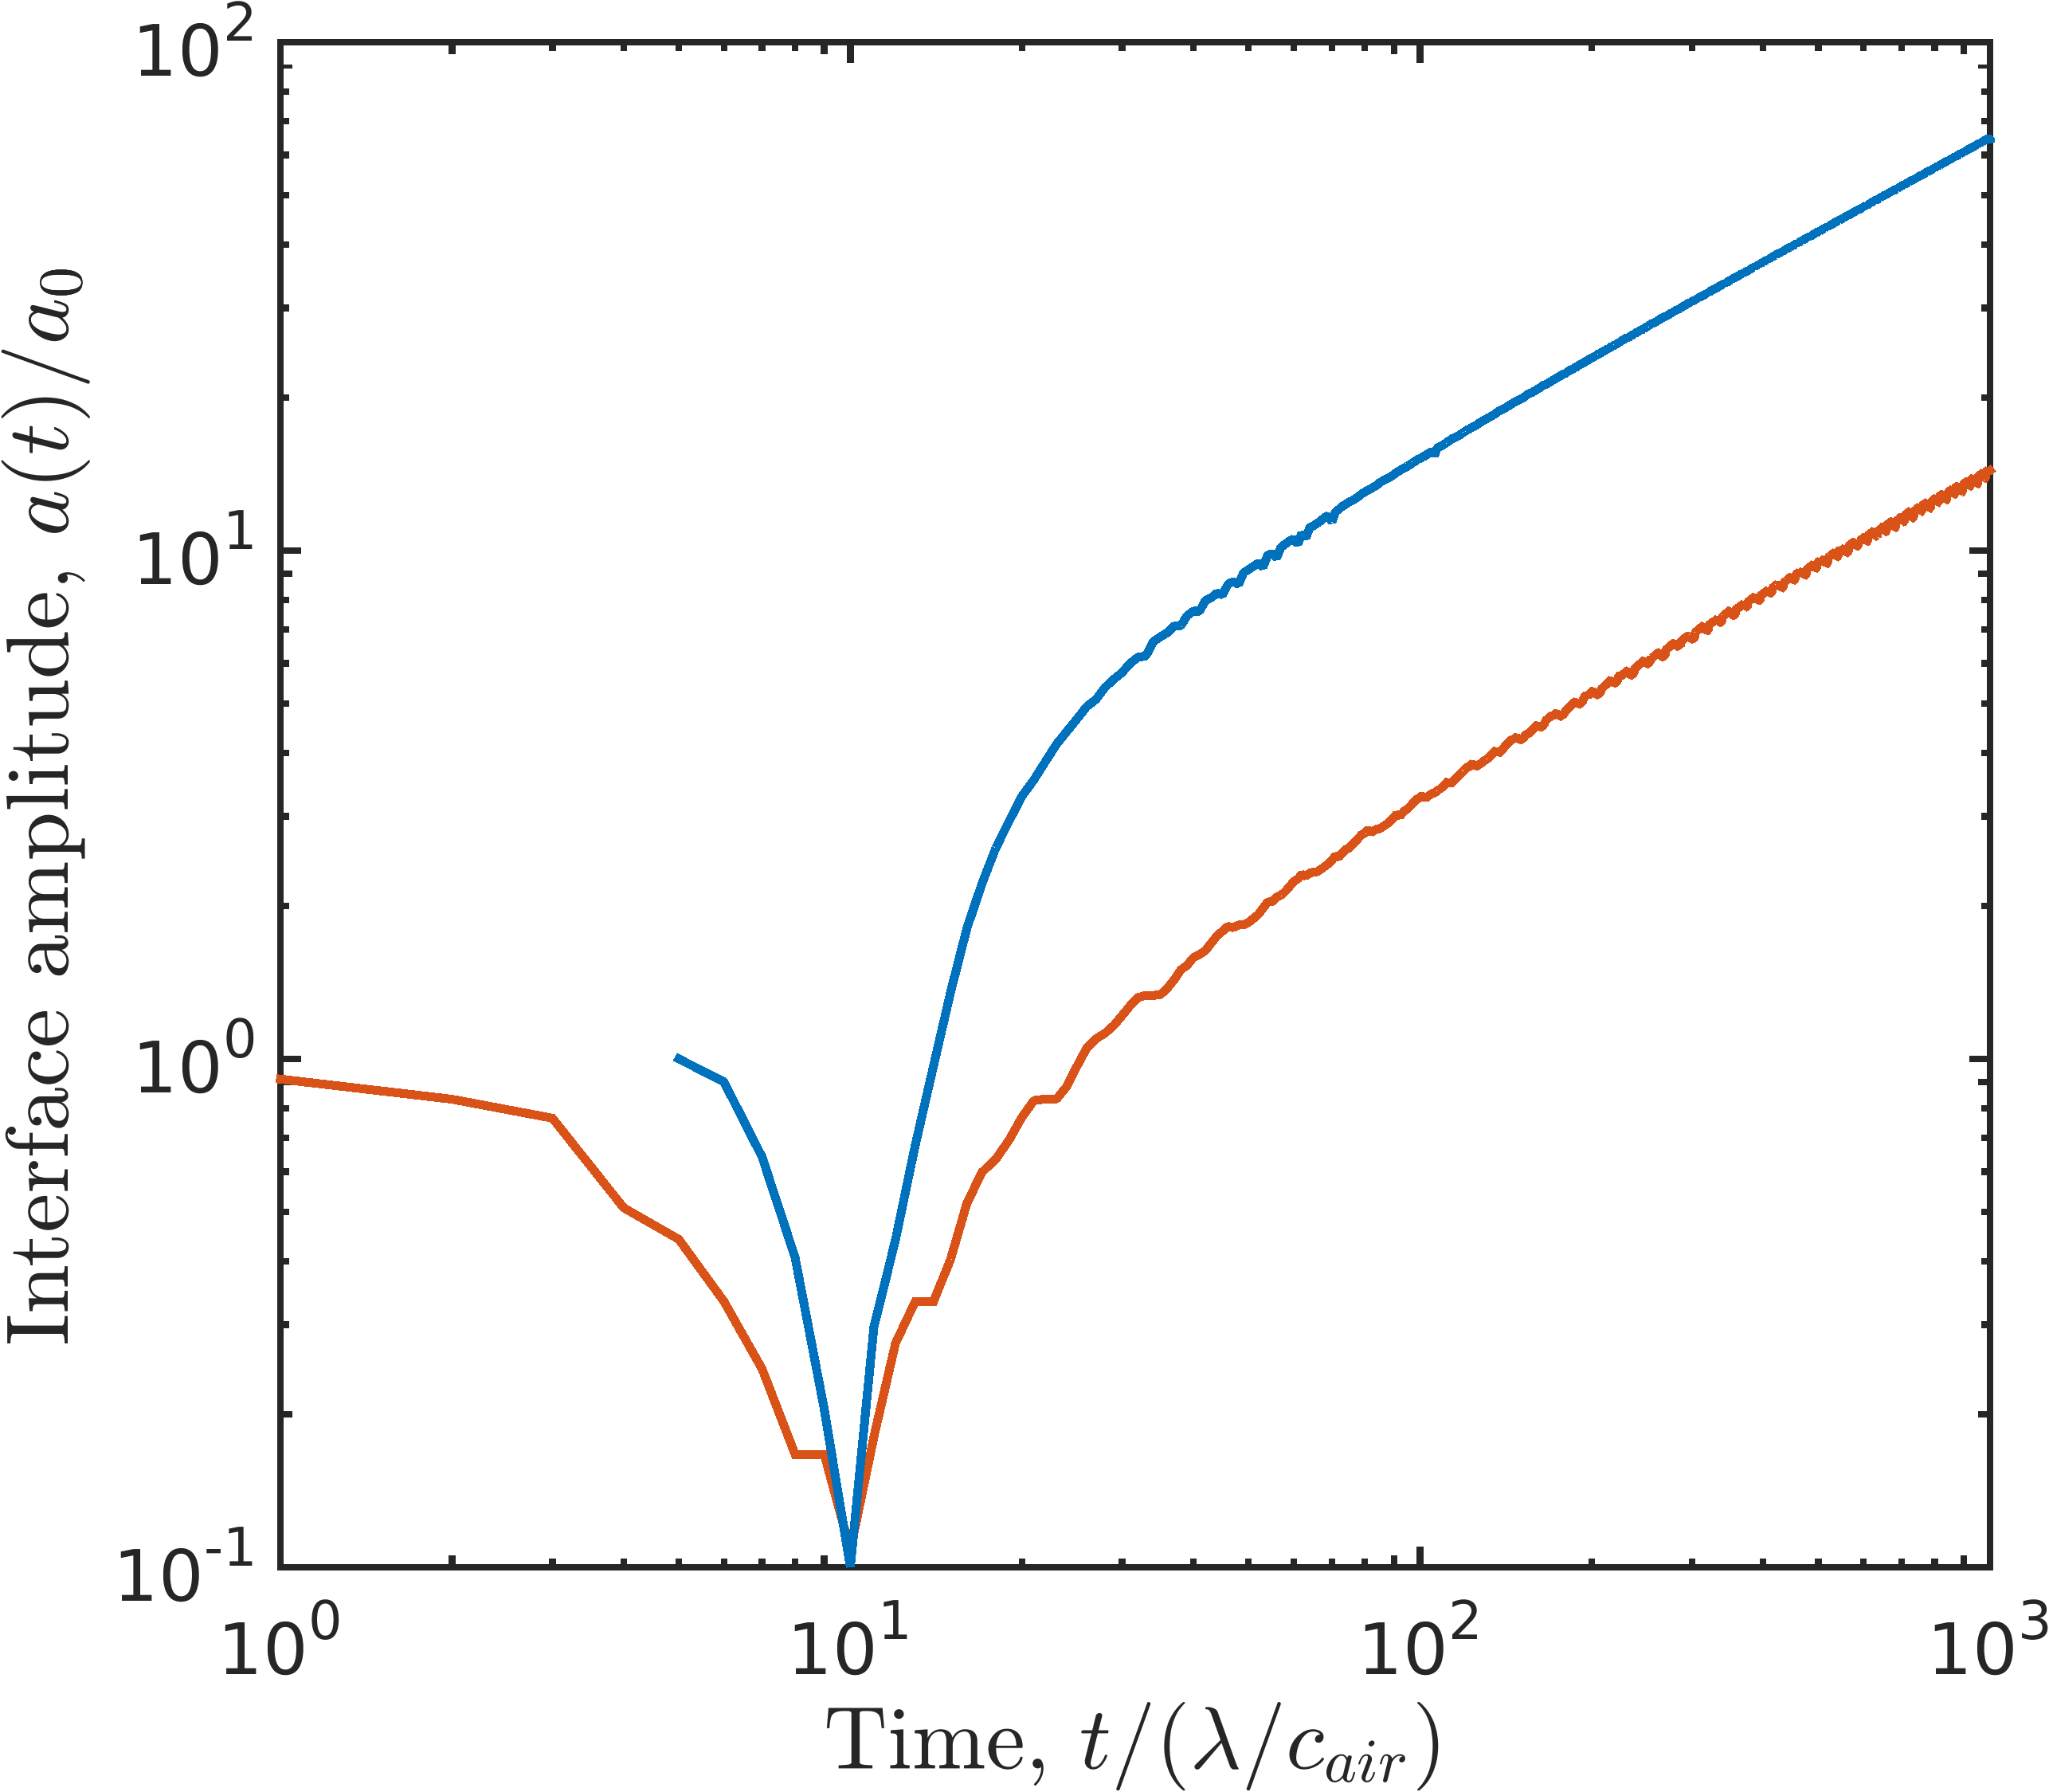
\includegraphics[width=0.6\textwidth]{../figs/lung_figs/interface_multi-amp_loglog_roe_t1000_nolines}%
      };%
      \begin{scope}[x={(image.south east)},y={(image.north west)}]%
        \node[font=\footnotesize,right] at (0.4,0.7){ $10$ MPa};%
        \node[font=\footnotesize,right] at (0.6,0.4){ $5$ MPa};%
      \end{scope}%  
    \end{tikzpicture}%
  \end{figure}
  \begin{center}
    We suspect vorticity is driving this late time growth.
  \end{center}
\end{frame}
%%% Local Variables:
%%% mode: latex
%%% TeX-master: "../main"
%%% End:
